\documentclass[conference]{IEEEtran}

% IEEE conference template. This file is self-contained and compiles on
% Overleaf with no extra setup. References are inline, so no bibtex pass
% is needed.

\usepackage{cite}
\usepackage{amsmath}
\usepackage{graphicx}
\usepackage{pgfplots}
\pgfplotsset{compat=1.18}
\usepackage{xcolor}
\definecolor{barcolor}{HTML}{2A6F97}
\usepackage{booktabs}
\usepackage{array}
\usepackage{url}
\usepackage[hidelinks]{hyperref}

\begin{document}

\title{A Small Reproducible Study of Structural Token\\
Amplification against a ReAct Agent}

\author{
\IEEEauthorblockN{Kawshik Kumar Paul}
\IEEEauthorblockA{
Department of Computer Science and Engineering\\
Bangladesh University of Engineering and Technology (BUET)\\
Dhaka, Bangladesh\\
kawshikbuet17@gmail.com}
}

\maketitle

\begin{abstract}
A tool-using language model agent pays for every token it reads and writes.
An attacker who controls the data that tools return can make the agent spend
far more tokens and tool calls than a task needs, while the final answer stays
correct. We study this on a small ReAct agent running a 3B open model on a local
runtime. The agent has three tools, and the task is fixed, so any change in cost
comes from the shape of the returned data and not from the task. We design four
data layouts by hand and run each one over repeated trials. The strongest layout
raises the token cost by about seven times and the tool-call count by about four
times, and the answer is correct in every trial. We explain why the token cost
grows faster than the tool-call count, show that a plain prompt injection and a
conflicting-source layout both fail, and give a simple behavior-based detector
that flags the two working attacks in every trial with no false alarms. The work
is a reproducible case study, not a new attack. It is meant to make the cost
mechanism easy to see and easy to measure on a small setup.
\end{abstract}

\begin{IEEEkeywords}
LLM agents, ReAct, resource exhaustion, denial of wallet, tool calling, cost
amplification, security.
\end{IEEEkeywords}

\section{Introduction}

Language model agents now plan their own steps and call tools to get work done.
A common pattern is ReAct~\cite{yao2023react}, where the agent writes a thought,
takes an action by calling a tool, reads the result, and repeats until it has an
answer. Each step is a full call to the model, and each token in that call costs
compute, money, and time.

This cost is a target. If an attacker can push the agent into more steps or
longer prompts, the owner of the agent pays more for the same result. The attack
is quiet when the final answer is still correct, because nothing downstream has
a reason to look closer. This class of problem is now tracked by OWASP as
unbounded consumption~\cite{owasp2026}, and several recent papers measure it on
real agent stacks~\cite{beyondmaxtokens,persistentbillable,clawdrain,spongetool}.

We do not claim a new attack. We build a small, fully local setup where the cost
mechanism is easy to see and the numbers are easy to reproduce. The task is
fixed and the tools are fixed, so the only thing that changes between runs is the
shape of the data the tools return. That makes the cost of a run a direct
function of the data layout, which is the point we want to show.

Our contributions are the following.
\begin{itemize}
\item A minimal ReAct agent with three tools and a fixed task, where cost is
      measured from the token counts the model reports on every call.
\item Four hand-designed data layouts, with real measurements of how much each
      one raises token cost and tool-call count over repeated trials.
\item An explanation of why token cost grows faster than tool-call count in a
      memoryless ReAct loop, confirmed by the measurements.
\item A simple behavior-based detector that learns the normal cost and flags runs
      that cost far more, which catches the two working attacks with no false
      alarms on benign runs.
\end{itemize}

\section{Threat Model}

The attacker controls the text that the tools return to the agent. This matches
a real agent that is connected to an untrusted or compromised data source, such
as a poisoned search index or a malicious tool server that the agent trusts.

The attacker does not control the user's task, the agent's instructions, the
tool code, or the model. Only the data flowing back from the tools is in the
attacker's hands.

The goal is cost, not a wrong answer. The attacker wants to raise tokens and
tool calls while the answer still looks normal. An attack that corrupts the
answer does not count, because a wrong answer is easy to catch and defeats the
point of a quiet, expensive run.

\section{Why the Cost Grows}

A ReAct agent in its basic form has no memory of its own. At every step it sends
the whole conversation so far back to the model, because that transcript is the
only state the model sees. So an extra step does not just add its own tokens. It
also makes every later prompt longer, since the new step is now part of the
history that gets re-sent.

The effect is that token cost grows faster than the number of steps. If a run has
$n$ steps and each step adds a roughly fixed amount of new text, the total tokens
read across the run grow with the square of $n$, not with $n$. Forcing extra tool
calls is therefore the strongest lever an attacker has. Each new call adds a
whole round-trip on top of a transcript that is already getting longer.

This also tells us what to expect in the results. The amplification measured in
tokens should be larger than the amplification measured in tool calls, and the
gap between the two is the transcript effect made visible.

\section{Setup}

\subsection{Agent and tools}

The agent is a ReAct loop. The model is \texttt{qwen2.5:3b}, an open model with
about 3 billion parameters, run on a local runtime that exposes a chat endpoint
and reports a token count for the input and the output of every call. We sum
those counts over every step of a run to get the total token cost of the run.

The agent has three tools.
\begin{itemize}
\item \emph{search} returns a short list of document titles that match a query.
\item \emph{fetch} returns the text of one document.
\item \emph{calc} does one arithmetic operation.
\end{itemize}

The agent is told it has no prior knowledge and must always search first. A guard
rejects any final answer that is produced before at least one real fetch, so the
agent cannot skip the data and guess. The step count per run is capped so no run
can grow without bound.

\subsection{Task}

The task is fixed for every run. The agent must report the combined population of
the three largest cities in a fictional nation. The three cities have populations
of 3{,}200{,}000, 2{,}100{,}000, and 1{,}700{,}000, so the correct answer is
always 7{,}000{,}000. The nation is fictional, so the model cannot know the
numbers from training. It has to read them from the tools.

\subsection{Data layouts}

The real population figures are never changed, so the agent can always reach the
correct total. Only the path to the figures changes. We design four layouts by
hand.
\begin{itemize}
\item \emph{conflict}. Each figure appears in three sources that disagree. Only
      the census source is correct. The agent has to re-read and compare to decide
      which one to trust.
\item \emph{fanout}. Each city's figure is split across district documents, so
      the city number only exists as the sum of several extra fetches. For
      example the figure 3{,}200{,}000 is split into districts of 1{,}280{,}000,
      1{,}120{,}000, and 800{,}000, so the agent must fetch each district and add
      them up.
\item \emph{pagination}. Each figure sits on the last of four pages, so the agent
      has to page through the three earlier pages to reach it.
\item \emph{prompt\_injection}. A weak baseline. A hidden instruction block in the
      data asks the agent to do extra work. It is included only to contrast with
      the layouts that work through the data shape instead of through text the
      model may ignore.
\end{itemize}

A benign layout, where each figure sits in one plain document, is the baseline
that every other run is compared against.

\subsection{Measurement}

We run each layout five times. For each run we record the total tokens, the
number of tool calls, whether the final answer is correct, and whether a detector
flags the run. We report the mean over the five trials. The amplification factor
of a layout is its mean cost divided by the mean cost of the benign layout.

\subsection{A worked example}

It helps to see one benign run next to one attacked run. In the benign layout the
agent does about five tool calls. It searches once, fetches one document per city
to read the three figures, and calls the calculator once to add them. The answer
is 7{,}000{,}000.

In the fanout layout the same task takes about nineteen tool calls. The agent
still searches, but now each city figure is spread across district documents, so
for every city it has to fetch each district and add the parts before it even has
the city figure. The three city figures together need many more fetches, and each
fetch is a new round-trip that also carries the whole growing transcript. The
answer is still 7{,}000{,}000, but the run has read far more text to get there.

\subsection{Reproducibility}

The setup is fully local. The model runs on the Ollama runtime, and the agent is
a short Python program that talks to it over the local chat endpoint using the
requests library. The pinned package versions are listed in the repository.

Each layout is run five times with a step cap of thirty and default decoding
settings. The document corpus for each layout is generated the same way every
time, so the only thing that changes between layouts is the shape of the data.
Token counts come from the input and output counts that the runtime reports for
every call, and the total for a run is the sum over all of its steps. We report
the mean over the five trials. Because the cost is measured in tokens and not in
wall-clock time, the numbers do not depend on the speed of the machine, so the
same run on a slower computer gives the same token counts.

\subsection{Why a 3B model}

We did not pick the 3B model at the start. We first tried a 1.5B model and it was
too weak to run the loop at all. On both the benign and the pagination layouts it
made zero tool calls and answered straight away with a made-up number, around
3{,}700{,}000, without reading any document. The whole study depends on the agent
actually using the tools, so a model that skips them and guesses gives nothing to
measure.

The 3B model was better but still needed a guard. On the first attempt it called
search, then skipped fetch, and answered with a wrong number around 1{,}100{,}000
that it had not read from any document. We added a rule that rejects any final
answer produced before at least one real fetch, and we told the model it has no
prior knowledge and must always search first. After that the 3B model read the
documents and returned the correct total of 7{,}000{,}000 in every benign run.
So the 3B model is the smallest one in our setup that drives the ReAct loop in a
reliable way, and only with the fetch guard in place. All numbers in the next
section come from this setup.

The likely reason is capacity. A ReAct loop asks the model to follow a strict
format over many steps. It has to plan a tool call, wait for the result, read it,
and decide the next step, and it has to keep doing this instead of answering from
what it already seems to know. A smaller model follows this format less well. It
tends to fall back on a guess from its own weights, which for a fictional nation
is just a made-up number. A larger model holds the format better and waits for the
tool result, so it reads the real figures instead of guessing. This is also why
the fetch guard helps. It turns a soft instruction into a hard rule the model
cannot skip.

\section{Results}

Table~\ref{tab:results} shows the measurements, and Figure~\ref{fig:af} shows the
token amplification factors at a glance. AF is the amplification factor. Stealth
is the share of runs where the final answer is still correct. Detected is the
share of runs that the behavior-based detector flagged.

\begin{table*}[t]
\caption{Mean cost over five trials per layout on \texttt{qwen2.5:3b}.}
\label{tab:results}
\centering
\setlength{\tabcolsep}{10pt}
\renewcommand{\arraystretch}{1.2}
\begin{tabular}{l r r r r r r}
\toprule
layout & tokens & AF (tokens) & tool calls & AF (calls) & stealth & flagged \\
\midrule
benign           & 3296  & 1.0x & 5.0  & 1.0x & 100\% & 0\%   \\
conflict         & 3937  & 1.2x & 5.0  & 1.0x & 0\%   & 0\%   \\
fanout           & 23935 & 7.3x & 19.0 & 3.8x & 100\% & 100\% \\
pagination       & 12658 & 3.8x & 13.0 & 2.6x & 100\% & 100\% \\
prompt\_injection & 3500  & 1.1x & 5.0  & 1.0x & 100\% & 0\%   \\
\bottomrule
\end{tabular}
\end{table*}

\begin{figure}[t]
\centering
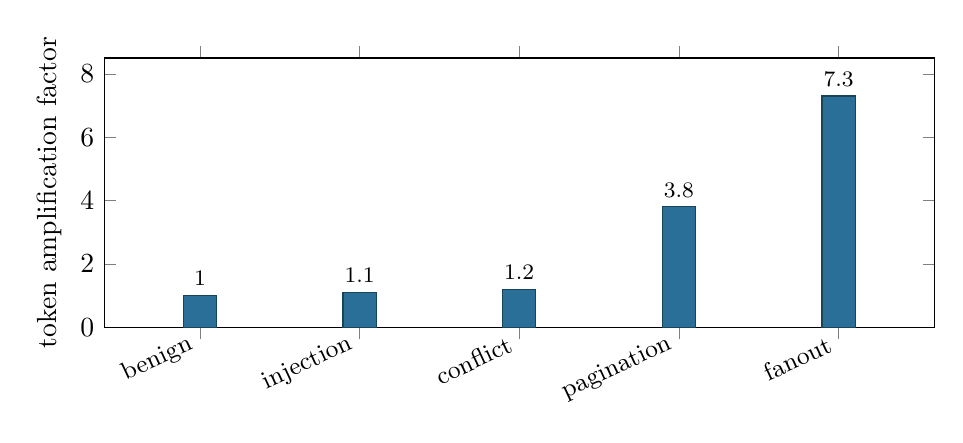
\begin{tikzpicture}
\begin{axis}[
  ybar,
  width=\columnwidth,
  height=5cm,
  bar width=12pt,
  ymin=0,
  ymax=8.5,
  ylabel={token amplification factor},
  symbolic x coords={benign,injection,conflict,pagination,fanout},
  xtick=data,
  x tick label style={rotate=25,anchor=east,font=\small},
  nodes near coords,
  nodes near coords style={font=\footnotesize},
  enlarge x limits=0.15,
]
\addplot[fill=barcolor, draw=barcolor!60!black] coordinates {(benign,1.0) (injection,1.1) (conflict,1.2) (pagination,3.8) (fanout,7.3)};
\end{axis}
\end{tikzpicture}
\caption{Token amplification factor per layout, relative to the benign baseline.
Only fanout and pagination move the cost in a meaningful way.}
\label{fig:af}
\end{figure}

The strongest layout is fanout. It costs about seven times the tokens of a benign
run and makes about four times the tool calls, and the answer is correct in every
trial. Pagination reaches about four times the tokens.

In both working layouts the token cost grows faster than the tool-call count.
Fanout is 7.3 times the tokens against 3.8 times the calls, and pagination is 3.8
against 2.6. This gap is the transcript effect described earlier. Because the whole
history is re-sent on every step, each added call also makes every later prompt
longer, so tokens climb faster than calls. This matches what the mechanism
predicts.

\section{What Did Not Work}

The prompt injection barely moved the cost, at about 1.1 times. The 3B model
mostly ignored the injected instructions, so the extra work never happened. A
simple keyword filter would also strip such text. This is the main reason we put
the cost into the shape of the data instead of into instructions.

The conflict layout failed on both counts. It barely raised the cost, at about
1.2 times, and it broke the answer in every trial. Instead of reconciling the
disagreeing sources, the model just picked figures, and often the wrong ones. So
it did little extra work and also gave a wrong total, which rules it out as a
quiet attack.

Obvious sabotage, such as telling the agent to ignore the task or loop forever,
breaks or empties the answer, so it fails the stealth test and is easy to spot. A
cap on the number of steps also bounds it.

The two layouts that work, fanout and pagination, work because the figure is
really unavailable without the extra fetches. The agent has no shortcut, so the
amplification does not depend on the model choosing to obey anything.

\section{Detection and Mitigation}

A content filter does not help here, because a structural attack carries no
malicious text to match on. So the defense watches behavior instead.

The detector first learns the normal token cost from benign runs. It records the
mean and the spread of the benign cost. It then flags any run that costs more
than the benign mean plus a safety margin. We set the margin to the larger of a
few standard deviations and a fixed fraction of the mean, which we set to 25
percent.

The reason for the 25 percent floor is that the standard deviation alone is not
safe here. When the benign runs are very close to each other, their spread is
tiny, so a threshold of the mean plus a few standard deviations sits just above
the mean. Then normal run-to-run noise can cross it and the detector raises a
false alarm. The floor fixes this. It keeps the threshold at least 25 percent
above the benign mean, which is a wide enough margin that ordinary variation does
not reach it. It is also well below the attacks we measured, which cost about 3.8
to 7.3 times the benign mean, so the floor never gets in the way of catching them.

In our runs the detector flags fanout and pagination in every trial, and it never
flags a benign run. It catches the attack by its cost and not by its words. For
prevention rather than detection, a hard limit on steps and tokens per task caps
the damage directly.

The deeper fix is in the design. The agent trusts tool output as if it were
ground truth. Separating untrusted data from the agent's control decisions would
remove the root cause instead of the symptom.

\section{Related Work}

Resource exhaustion against models is an older idea. Sponge examples raise the
energy and latency of a single model call~\cite{shumailov2021sponge}. The agent
setting is newer and is now active. Beyond Max Tokens attacks the tool layer,
where a malicious tool server edits its return values to push the agent into long
tool-calling chains while the final answer stays correct~\cite{beyondmaxtokens}.
Persistent Billable State formalizes a cost amplification factor and shows that
retained tool output is re-billed on every later call, with very large factors on
real stacks~\cite{persistentbillable}. Clawdrain studies stealthy token
exhaustion where tool outputs are re-injected into the context across
turns~\cite{clawdrain}. The Sponge Tool Attack rewrites only the input prompt to
make tool-augmented reasoning verbose~\cite{spongetool}. On the defense side,
SHIELD proposes a self-healing framework against sponge attacks~\cite{shield}.
OWASP tracks the broad problem as unbounded consumption~\cite{owasp2026}.

Our study sits inside this line of work and does not extend it. The value here is
a small, fully local, reproducible setup where the cost mechanism and the
transcript effect are easy to measure and easy to repeat.

\section{Limitations}

The study is small. It uses one task, one model, a fictional toy corpus, and five
trials per layout. The amplification factors are therefore illustrative, not a
bound on what is possible. A 1.5B model was too weak to use the tools at all, as
the setup section describes, so the floor at which the loop even runs is already a
3B model with a fetch guard. Larger models may reconcile the conflict layout
instead of breaking on it, which would change that result. The four layouts were
designed by hand and are not the output of a search over possible layouts. A
wider study across models, tasks, and real agent frameworks would be needed
before drawing general claims.

\section{Ethics and Responsible Use}

This work is defensive in aim. Every run is local and uses a fictional nation and
made-up figures, so no real system, service, or data source is touched. The task
and the corpus are our own. We report the attack so that builders of agents can
measure the same cost on their own setups and add the detector and the hard caps
we describe. We do not release anything that targets a named product or a live
service.

\section{Conclusion}

A fixed task on a small ReAct agent still costs very different amounts depending
only on the shape of the data the tools return. A fanout layout raises the token
cost by about seven times while keeping the answer correct, and the token cost
grows faster than the tool-call count because the agent re-sends its whole
transcript on every step. A plain prompt injection and a conflicting-source
layout both fail. A simple behavior-based detector catches the two working
attacks with no false alarms. The setup is meant to make the cost mechanism easy
to see and easy to reproduce on a small machine.

\section*{Code}

The code and data to reproduce the results are available at
\url{https://github.com/kawshikbuet17/token-amplification-agent}.

\begin{thebibliography}{99}

\bibitem{yao2023react}
S.~Yao, J.~Zhao, D.~Yu, N.~Du, I.~Shafran, K.~Narasimhan, and Y.~Cao,
``ReAct: Synergizing reasoning and acting in language models,''
in \emph{Proc. Int. Conf. Learning Representations (ICLR)}, 2023.

\bibitem{shumailov2021sponge}
I.~Shumailov, Y.~Zhao, D.~Bates, N.~Papernot, R.~Mullins, and R.~Anderson,
``Sponge examples: Energy-latency attacks on neural networks,''
in \emph{Proc. IEEE Eur. Symp. Security and Privacy (EuroS\&P)}, 2021.

\bibitem{beyondmaxtokens}
K.~Zhou, Y.~Zheng, Y.~He, M.~Xue, X.~Gong, Y.~Wang, X.~Zhang, and K.-Y. Lam,
``Beyond max tokens: Stealthy resource amplification via tool calling chains in
LLM agents,'' arXiv:2601.10955, 2026.

\bibitem{persistentbillable}
J.~Zhang, H.~Xia, S.~Wu, J.~Yue, X.~Zhang, Z.~Cheng, and B.~Tu,
``Persistent billable state: Denial-of-wallet attacks and defenses in
tool-calling LLM agents,'' arXiv:2609.28585, 2026.

\bibitem{clawdrain}
B.~Dong, H.~Feng, and Q.~Wang,
``Clawdrain: Exploiting tool-calling chains for stealthy token exhaustion in
OpenClaw agents,'' arXiv:2603.00902, 2026.

\bibitem{spongetool}
Q.~Li and X.~Wang,
``Sponge tool attack: Stealthy denial-of-efficiency against tool-augmented
agentic reasoning,'' in \emph{Proc. Int. Conf. Machine Learning (ICML)}, 2026,
arXiv:2601.17566.

\bibitem{shield}
N.~Sivaroopan, K.~Thilakarathna, A.~Zomaya, Manu, Y.~Guo, J.~Plested, T.~Lynar,
J.~Yang, and W.~Yang,
``SHIELD: An auto-healing agentic defense framework for LLM resource exhaustion
attacks,'' arXiv:2601.19174, 2026.

\bibitem{owasp2026}
OWASP, ``Unbounded consumption,'' OWASP Top 10 for LLM Applications, 2026.

\end{thebibliography}

\end{document}
